\documentclass[a4paper,english, 11pt]{article}


\usepackage[utf8]{inputenc}
\usepackage[T1]{fontenc}
\usepackage{lmodern} 
\usepackage{xcolor}
\usepackage{parskip} 
\usepackage{amssymb,amsthm,framed}  
\usepackage[]{amsmath} 
\usepackage[hang,small,bf]{caption}
\usepackage{siunitx} 
\usepackage{bm}
\usepackage{url}  
\usepackage{multirow} 
\usepackage[hidelinks]{hyperref}
\usepackage[a4paper,inner=2.5cm,outer=2.5cm,top=2.5cm,bottom=2.5cm,pdftex]{geometry} 

%  
\usepackage{listings}
\lstset{language=bash}
\lstset{basicstyle=\ttfamily,
  numbers=left,
  showstringspaces=false,
  commentstyle=\color{red},
  keywordstyle=\color{black},
  breaklines=true,
  belowskip=0.5em
}


\usepackage{accsupp}    
\lstset {
    numberstyle=\noncopynumber,
    columns=flexible,
}

\newcommand{\noncopynumber}[1]{
    \BeginAccSupp{method=escape,ActualText={}}
    #1
    \EndAccSupp{}
}


\usepackage{graphicx}     

\usepackage{enumitem}      
\graphicspath{{../Images/}} 
 
\hyphenpenalty=5000
\tolerance=1000
\title{Draft: The Nansen Legacy labeling manual}
\date{\today\\v0.1}
\author{Pål Ellingsen (\url{pale@unis.no})}

\begin{document}
\maketitle
\tableofcontents
\section{Introduction} % (fold) {{{
\label{sec:Introduction}

The Nansen Legacy project is aimed at generating samples, data and science relevant during the project and after its conclusion. Additionally it is a collaboration between major marine institutions in Norway. To accommodate the tracking of samples between from ship to land and  between institutions it was decided to use a unified labeling system. To secure that the project data and metadata follows the FAIR (Findable, Accessible, Interoperable, Reproducible) principle for data management within the project, a first step is to ensure that the collected samples are findable and that relevant metadata are logged
along with the sample collection. The metadata needs to be logged in a standardized manner and will be
made accessible through a search interphase as soon as possible after the cruises.  This manual details how to label samples, log the metadata and how to find information about logged samples in the SIOS database.  

% section Introduction (end) }}}

\section{Labeling samples} % (fold) {{{
\label{sec:Labeling samples}



In order to be able to distinguish samples, samples in the project are assigned a unique id, in the form of a universally unique identifier (UUID). Details about it can be found in subsection~\ref{sub:UUID}. For physical samples this UUID is encoded in the form of a 2D barcode, specifically a Data Matrix (DM) code, details in subsection~\ref{sub:DM}. An example of such a code can be seen in figure~\ref{fig:data_matrix}. The code is then printed, together with descriptive text, onto a label which is stuck on the sample or its container.

\begin{figure}[htb]
    \centering
    
\includegraphics[width=0.1\textwidth]{Data_matrix.png}
    \caption{\label{fig:data_matrix}
        Example Data Matrix code containing an UUID.
    }
\end{figure}

\subsection{Procedure for physical samples} % (fold) {{{
\label{sub:Procedure for physical samples}


The interface for printing labels is available through a webpage on the research ship. Details of this is given by the cruise leader.

\begin{enumerate}
    \item Choose label size.
    \item Write information which is to be printed together with the label into the printing page. This should include the date and information about what the sample is.
    \item Print the label.  
\end{enumerate}
The following steps can be done in any order depending on what is easiest:
\begin{enumerate}
\setcounter{enumi}{3}
    \item Stick the label on the sample
    \item Register data about the sample in the spreadsheet, see section~\ref{sub:spreadsheet_reg}.
\end{enumerate}

% subsection Procedure for physical samples (end) }}}

\subsection{Procedure for virtual samples} % (fold) {{{
\label{sub:Procedure for virtual samples}

Examples of virtual sample are: gear casts, Multicores, Multinets and Ice cores that have been split/melted. Since these have no physical place for a label to go, the procedure of logging them involves either printing a sheet of paper with the codes or just assigning them a UUID without any Data Matrix code. Which approach is the best depends on the circumstance. If the UUID is going to be used by more than one scientist, for example in the case of Niskin bottles, it is often easier to print an A4 page with the codes. Below follows two different procedures depending on what is chosen:

\subsubsection{A4 page of codes} % (fold) {{{
\label{ssub:A4_page}

Go to the ''Gear UUID generator'' page on the printing overview (address distributed on the cruise). 
On this page you specify the name of the gear ''Gear Name'' (CTD, Multinet, Multicorer), the type of container ''Sample Name'' (Niskin, core, net), number of samples in on gear cast ''Number of samples'' and number of gear casts expected ''Number of pages'' (this is only to save having to come to this page for every cast). 

By pressing ''Make PDF'' a PDF is generated and can be printed on an normal printer. The A4 page printed should be marked with information identifying which gear cast this is for. Then all the containers need to registered in the same way physical samples are, see subsection~\ref{sub:spreadsheet_reg}.

\textbf{Note: It is very important that one person is responsible for registering the containers, as without them samples will be without parents and untraceable.}

If copies are needed for several scientists to work on the same containers, the A4 page can be copied on a copier. 

% subsubsection A4_page (end) }}}

\subsubsection{Only UUID} % (fold) {{{
\label{ssub:Only_UUID}

When only the UUID is needed, one can be generated through the ''UUID generator'' on the printing overview. Pick one of them and continue the registration as in subsection~\ref{sub:spreadsheet_reg}. Remember to ''Get new UUID'' for every time you leave the page in order to ensure that a UUID is used twice.  

% subsubsection Only_UUID (end) }}}
% subsection Procedure for virtual samples (end) }}}

\subsubsection{Hierarchy} % (fold) {{{
\label{sub:Hirarcy}

By using UUIDs for the samples it will be possible to keep track of the hierarchy of the samples. By issuing a new UUID for each subsample, and linking it with the sample UUID, one can easily track the hierarchy. How this would be done is shown in figure~\ref{fig:parent_uuid}.
\begin{figure}[htb]
    \centering
    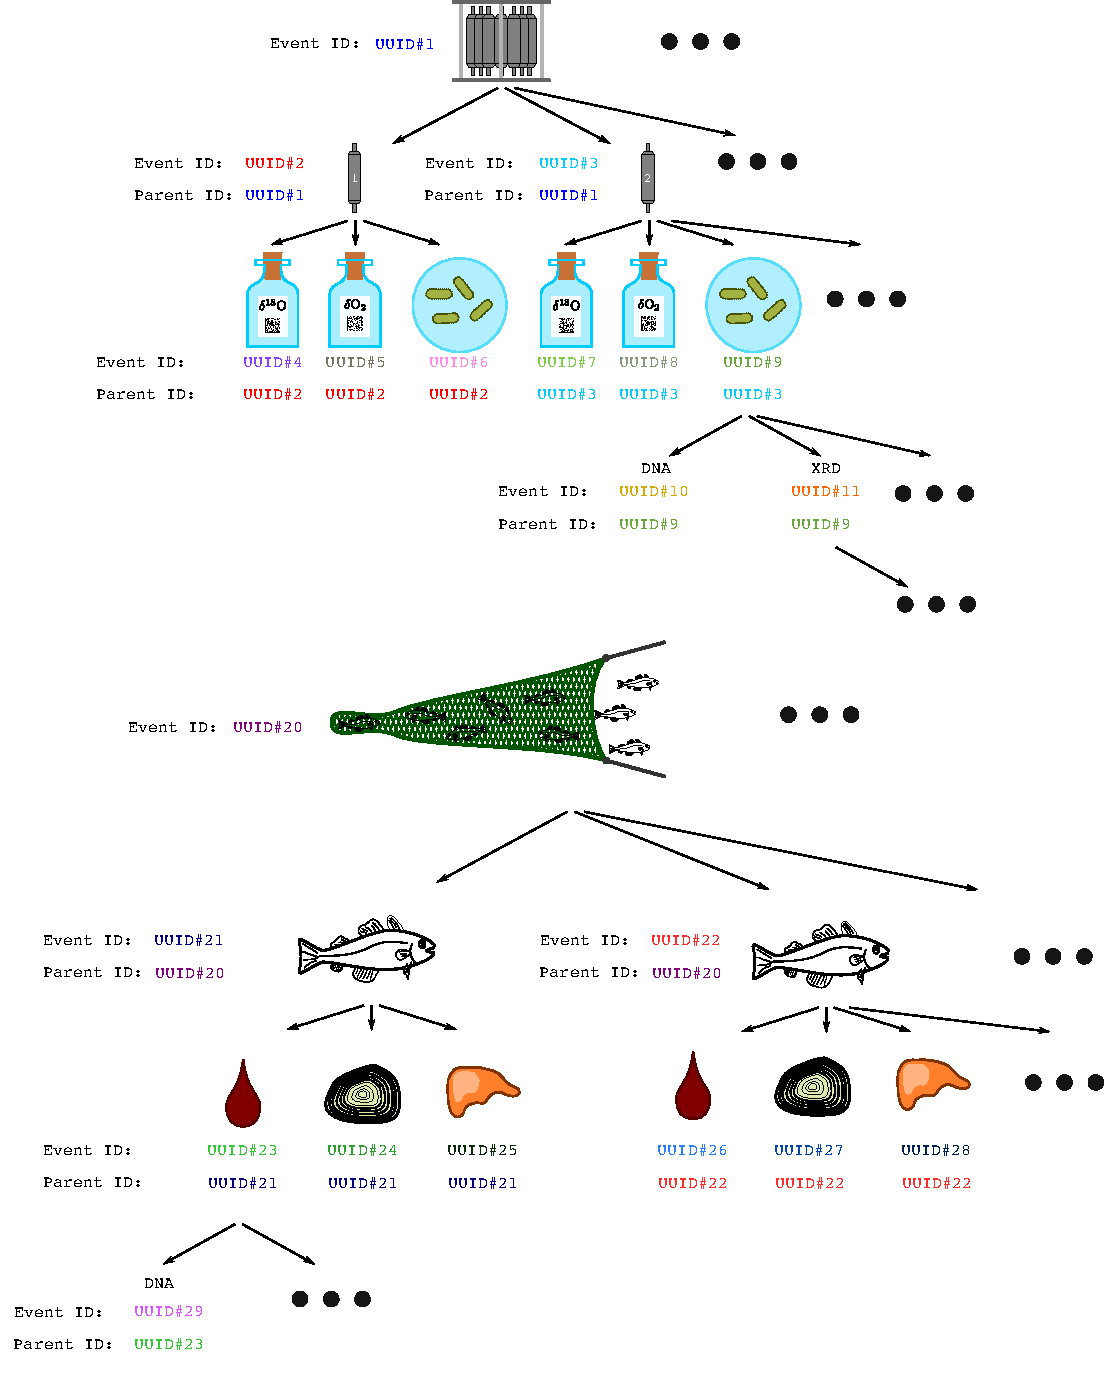
\includegraphics[width=1\textwidth]{Labeling.pdf}
    \caption{\label{fig:parent_uuid}
       Examples of how event id and parent id works for two different gear types. These should be transferable to other gear types.
    }
\end{figure}
% subsection Hirarcy (end) }}}
In order to 

\subsection{Generation of sample log spreadsheet} % (fold) {{{
\label{sub:Sample_log_spreadsheet_generation}

% subsection   (end) }}}

\subsection{Sample logging} % (fold) {{{
\label{sub:spreadsheet_reg}


The samples taken during a cruise need to be logged in a standardised spreadsheet, see subsection~\ref{sub:Sample_log_spreadsheet_generation} for how to make one. Logging of samples should be done continuously during the cruise. 

When logging the sample you will need its id, for physical samples this id goes in the Sample ID field and should be entered by scanning the Data Matrix code on the sample label. Then its parent needs to be registered, what the parent is depends on what type of sample it is, see figure~\ref{fig:parent_uuid} for some examples. Having registered these two, the rest of the columns in the spreadsheet needs to be filled out. Every column has an explanation of what is expected in the given field. 


% subsection Sample log spreadsheet logging (end) }}}
\subsection{Labels} % (fold) {{{
\label{sub:Labels}

The labels for the samples need to be printable in the field and fit on different size containers. So far it has been identified that there is a need for two sizes of labels, one for Eppendorf tubes (2 ml) and one for larger containers.

\subsubsection{Eppendorf labels} % (fold) {{{
\label{ssub:Eppendorf labels}

These labels need to withstand temperatures down to \SI{-196}{\degree\celsius} and up to \SI{100}{\degree\celsius}. In addition, they need to be resistant to laboratory solvents and water. Once attached the labels should be hard to remove, as they will contain the unique identification for the sample.

So far it looks like CILS international has some labels which wrap around the Eppendorf tube, with a printable area (with a thermal printer) of \SI{25x19}{\mm}. There are also labels available from Sigma Aldrich.


% subsubsection Eppendorf labels (end) }}}

\subsubsection{Larger labels} % (fold) {{{
\label{ssub:Larger labels}
These labels are for the use on larger samples, and should withstand temperatures in the range of \SIrange{-80}{100}{\degree\celsius}, laboratory solvents and water. These should be hard to remove as they contain the unique identification for the sample.

CILS size is \SI{26x79}{\mm}

CILS and Sigma Aldrich can both supply labels that suite this, though CILS seems to have a higher standard.
% subsubsection Larger labels (end) }}}
% subsection Labels (end) }}}

\subsection{Printer} % (fold) {{{
\label{sub:Printer}
To ensure that the labels can be printed in the field and that the marking stays on, thermal printers should be used. The easiest is to have one printer for each size of the label. In addition to printing the Data Matrix code, these printers will be able to add information from each scientist in human readable format (text), helping to identify the sample without the need to scan it each time.

For this it looks like a \emph{Zebra GX430t}, see figure~\ref{fig:zebra}, will satisfy the requirements. This printer supports printing using ZPL codes and Data Matrix codes following ECC 200, which then means that a custom (Python) program can be used to generate the needed UUID and add the text wanted from the scientist. Here an API to pull the cruise number of the boat would be advantageous. 
% subsection Printer (end) }}}

In operation the printer uses ribbon, which needs to periodically be changed, though this is not a large running cost.
\subsection{Scanner} % (fold) {{{
\label{sub:Scanner}

Data Matrix codes can be read with a smartphone or webcamera, though this is not a robust solution, as the needed information should be easily inserted into an Excel sheet / database search. A faster and better solution is to use a hand held imaging barcode reader. It needs to be robust for use in the field, and easily interfaced to the computer.

A reader that satisfies this is the \emph{Datalogic PowerScan PD9530-DPM}, see figure~\ref{fig:scanner}. It is suited for reading small Data Matrix codes, which is necessary as the codes on the Eppendorf tubes need to be small in order to avoid to large a distortion from the code being wrapped around the tube. 
% subsection Scanner (end) }}}

% section Marking samples (end) }}}
\appendix

\section{Technical details} % (fold) {{{
\label{sec:Technical details}

\subsection{UUID} % (fold) {{{
\label{sub:UUID}

\subsubsection{Generation} % (fold) {{{
\label{ssub:Generation}

The reason for using UUID (universally unique identifier) to mark samples is that given a good seed, the generation of UUIDs (with for example UUID1) ensures that the code is unique (the probability of collision is on the order of $ 2\times10^{-18}$). UUID1 contains the time and information about the computer generating it. This could be a good code to use for AeN as it contains the time of generation. UUID generation is implemented in most languages, and is easily done in for instance Python by importing the built in library \emph{uuid}. 

% subsection Generation (end) }}}

\subsection{Data Matrix} % (fold) {{{
\label{ssub:DM}
Samples are going to be marked with UUID hex codes, example \emph{dbad1808625f11e880faa0481c9e7d26}. As these contain 32 hex digits, it is impractical to manually type these. A good solution for marking and reading these is the use of Data Matrix codes following the ECC 200 standard. To fit the UUID the code will be of size  $22\times22$, see figure~\ref{fig:data_matrix} for an example.

% subsection Data Matrix (end) }}}

% section Technical details (end) }}}

\section{Costs} % (fold) {{{
\label{sec:Costs}

The cost of the purposed solutions are shown in table~\ref{tab:costs}.
\begin{table}[htb]
    
    \caption{\label{tab:costs}The unit costs}
    \begin{tabular}{lllrr}
        \hline
        \textbf{Item} & Need & \textbf{Unit size} & \textbf{Unit price} & \textbf{Total price} \\
        \hline
        CILS Eppendorf label    & 5 000     & Per label  (5 000)    & 2.16 NOK  & 10 800 NOK\\ 
        CILS Eppendorf label    & 20 000    & Per label  (20 000)   & 1.33 NOK  & 26 661 NOK\\ 
        CILS Larger label       & 5 000     & Per label  (5 000)    & 2.14 NOK  & 10 675 NOK\\ 
        CILS Larger label       & 20 000    & Per label  (20 000)   & 1.55 NOK  & 31 107 NOK\\ 
        Zebra GX430t            & 3         & Per unit              & 4950 NOK  & 14 850 NOK\\ 
        Zebra 2300 print ribbon & 3         & $12\times74$~m         & 320 NOK   & 960 NOK\\ 
        Datalogic PD9530-DPM    & 3         & Per unit              & 6478 NOK  & 19 434 NOK\\ 
        \hline
    \end{tabular}
\end{table}


Based the costs presented in the table and the initial needs (20 000 Eppendorf and 5 000 larger labels) the total cost comes to about \textbf{73 000 NOK}.
% section Costs (end) }}}

\end{document} 
